\documentclass{article}

\usepackage[nocompress]{cite}
\usepackage{graphicx}
\usepackage{geometry}
\usepackage{pdflscape}
\usepackage{amsmath}
\usepackage{url}
\usepackage{pgfgantt}
\usepackage{ragged2e}
\usepackage{caption}
\usepackage{verbatim}

\begin{document}
\newgeometry{vmargin=2.25cm, hmargin=2.25cm}
\title{Mathematical Model}

\author{Andrew Lamzed-Short}

\maketitle

\section{Mathematical Model}

In order to get a gist of the amount of reasonable work the GPU could handle at once and estimates for the amount of time and data movement needed for the optimal implementation, a mathematical model was developed to help visualise and describe the interactions between adjacent cells in the approximated algorithm that SNAP uses. The following assumptions were made when developing this model:

\begin{enumerate}

\item The algorithm defines the problem space as a three-dimensionality discretized grid of cells, each with their own values and interactions with their neighbouring adjacent cells – this forms the core of the SNAP algorithm (it itself approximating a continuous algorithm).

\item The problem space is cubic with side $ n $ for ease of modelling. A generalisation to a cuboidal space with dimensions $ (x, y, z) $ can be abstracted from the cubic model later.

\end{enumerate}

\begin{figure}[h!]
\centering
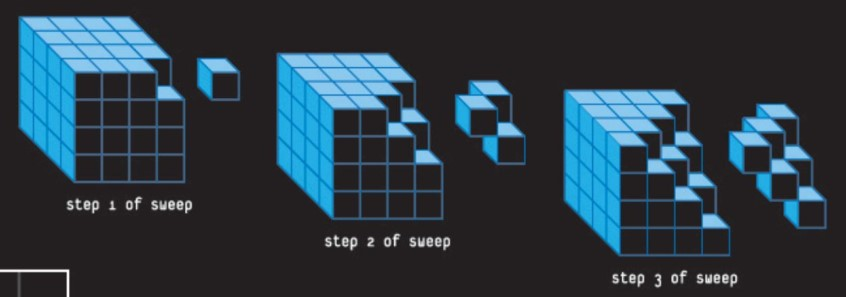
\includegraphics[width=0.45\textwidth]{images/Sweep.jpg}
\caption{Slices of a sweep of 3D grid}
\label{fig:3dsweepslice}
\end{figure}

Given these assumptions, we aim to derive the total number of communications between cells in the grid per iteration and how much work this equates to and how much can be parallelised at each stage.

There are $ 8 $ vertices of a cube so $ 8 $ octants to perform the sweep over. Each sweep is divided up into diagonal slices, shown in Figure \ref{fig:3dsweepslice}, of which there are $ (x + y + z) – 1 $ of them ($ 3n – 1 $ in this model). A key point to note is the dependency in each sweep of a slice on the slice before as the direction of the sweep is linear and calculations rely upon previous ones\footnote{As described in the documentation of the SNAP algorithm in their GitHub repository - \url{ https://github.com/lanl/SNAP/blob/master/docs/SNAP-overview-presentation-2015.pdf}}, and each combined sweep of all octants, after all results being collated, forms the basis of the next sweep.

The first $ n $ slices of the grid are comprised of the sum of the first $ n $ triangular numbers’ (i.e. $ 1, 3, 6, 10, 15… $)\footnote{Sequence A000217 in the ``On-line Encyclopedia of Integer Sequences'' (\url{https://oeis.org/A000217})}, worth of cells, with the final $ n $ slices having the same number also (just in reverse order). $ n - 2 $ slices exist between the 2 triangular-based pyramids formed from the previous step, allowing us to develop a function for the first $ m = n + \frac{n - 2}{2} $ slices, and mirror it to get the number of cells in any slice of the grid.

The number of cells in slice $ i $ of a cube of size $ n $ is thus given by the following formula:

\begin{equation}
cells(i) = \left\{
	\begin{array}{ll}
		tri(i) & \mbox{if } i \le n \\
		tri(i) - 3tri(i - n) & \mbox{if } i \le m \\
		cells(m - ((i - 1)\bmod m)) & \mbox{otherwise}
	\end{array}
\right.
\end{equation}

Where $ tri(i) $ represents the $i$th triangular number, $ 1 \le i \le 3n - 1 $. 

This means poor performance early on due to low numbers of cells per layer and the inter-slice dependency, but will ultimately scale well and to more graphics card given a large grid.

To work out data transfer, we need to figure out the amount of sends and receive actions are performed per slice. We can again work first out up to the first $ m $ slices, and take the mirror image for the rest of the slices, swapping the number of sends per slice for the receives of the mirror slice and vice versa. For the first $ n - 1 $ slices, each cell sends to 3 neighbouring adjacent cells in the next slice. When $ i \ge n $, we need to take into account the ``cut-off'' portions where some cells only send to 2 neighbours, hence:

\begin{equation}
sends(i) = \left\{
	\begin{array}{ll}
		tri(i) * 3 & \mbox{if } i < n \\
		(i\bmod(n - 1)) * 2 + \\
			(cells(i) - i\bmod(n - 1)) * 3 & \mbox{if } i \le m \\
		recvs(2n - i) & \mbox{otherwise}
	\end{array}
\right.
\end{equation}

The total number of receive actions is similar. The first cell has no neighbours to receive from, the second slice has only 1, the rest have three, then after the $n$th slice we need to consider where we only receive from 2 neighbours:

\begin{equation}
recvs(i) = \left\{
	\begin{array}{ll}
		0 & \mbox{if } i = 1 \\
		tri(i) & \mbox{if } i = 2 \\
		tri(i) * 3 & \mbox{if } i \le n \\
		(cells(i) - (2n - i)) * 3 & \mbox{if } i \le m \\
		sends(2n - i) \mbox{otherwise}
	\end{array}
\right.
\end{equation}

Both functions are defined in the domain $ 1 \le i \le 3n - 1 $.

If we let $ msg_s $ be the size of a message to send and $ msg_r $ the size of a message to receive from a neighbour (both in number of bytes), and knowing that the fastest data transfer rate of the PCI Express (PCIe) 2.0 bus connecting the graphics card and CPU together is 500MB/s\cite{PCIe}, we can calculate the time per slice to store data from the GPU as

\begin{equation}
time_s = \frac{sends(i) * msg_s}{5 \times 10^8}
\end{equation}

and to send data to it as

\begin{equation}
time_r = \frac{recvs(i) * msg_r}{5 \times 10^8}
\end{equation}

Aggregating these over all slices, alongside an assumed small, constant kernel function calculation time $ C $ over $ cells(i) $ cells in the slices, yields the best-case calculation time for the current approach. From here, we can interleave all 8 octants for calculation at once (of course managing the number of streaming multi-processors, which, after a point, we'd need to vastly scale hardware or queue work) to improve our throughput. $C$ ultimately depends on the type of graphics card being used.

\end{document}